\section{Aufbau und Durchführung}
\subsection{Aufbau}
\label{subsec:Aufbau}
Der Aufbau der Messapparatur ist in \autoref{fig:Aufbau} dargestellt. Eine Lichtquelle erzeugt Licht, das kollimiert und durch ein Interferenzfilter geschickt wird, welches nur die D1-Linie des 
Rb-Spektrums (λ = 794,8 nm) durchlässt. Aus dem unpolarisierten Licht wird durch einen Polarisationsfilter und eine λ/4-Platte zirkular-polarisiertes Licht erzeugt, das auf die Dampfzelle trifft.
Diese Dampfzelle kann erhitzt werden, um Rubidium-Dampfdruck zu erzeugen. Das durch die Dampfzelle hindurchtretende Licht wird auf ein Si-Photoelement fokussiert,
das über einen Linearverstärker an ein Oszilloskop angeschlossen ist. Schwankungen in der Lichtintensität führen zur Y-Auslenkung des Elektronenstrahls im Oszilloskop.\\
\begin{figure}[H]
    \centering
    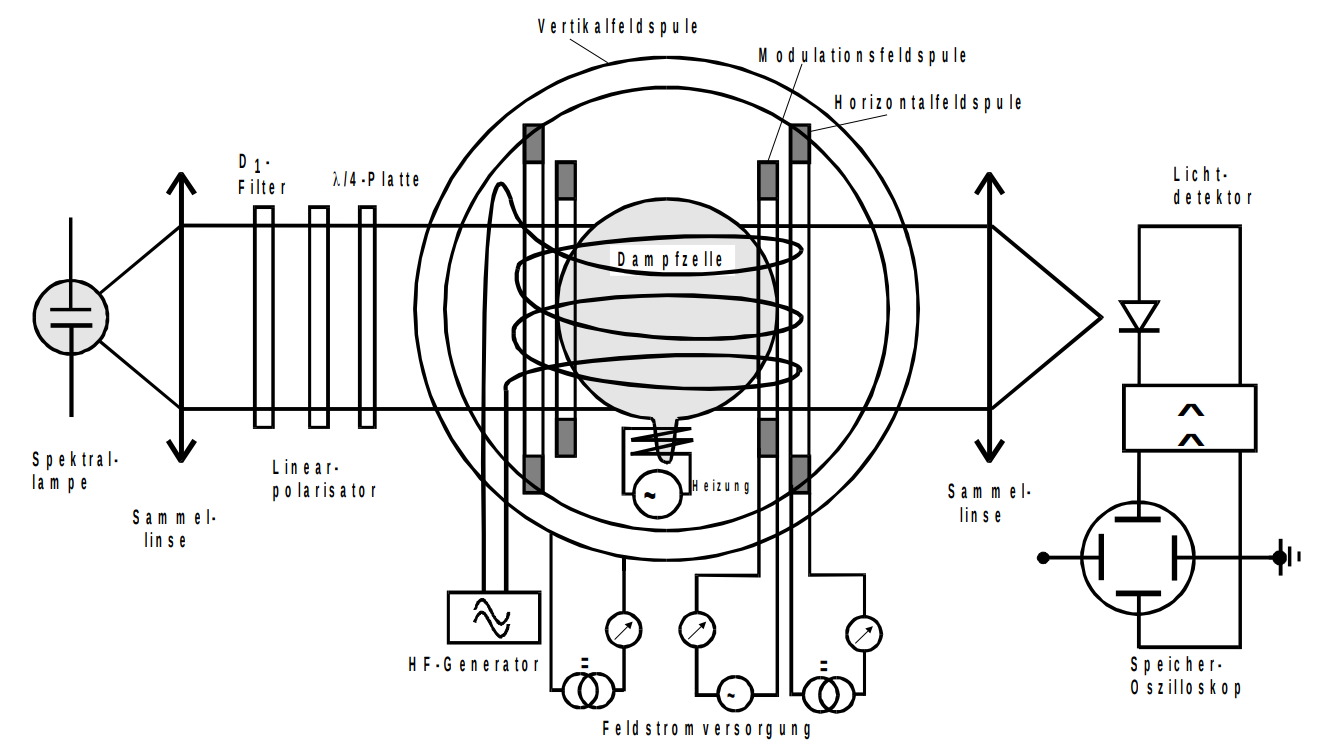
\includegraphics[width=0.7\textwidth]{images/aufbau.png}
    \caption{Schematischer Aufbau der Messapparatur. \cite{V21}}
    \label{fig:Aufbau}
\end{figure}

Der Versuchsaufbau verfügt über drei Helmholzspulenpaare:
\begin{itemize}
    \item Horizontalfeld-Spule: Mittlerer Radius R = 15,79 cm, Windungszahl N = 154
    \item Sweep-Spule (Modulationsfeldspule): Mittlerer Radius R = 16,39 cm, Windungszahl N = 11
    \item Vertikalfeld-Spule: Mittlerer Radius R = 11,735 cm, Windungszahl N = 20
\end{itemize}
Diese Spulen sind an das Kontrollgerät angeschlossen, das die Stromstärke in den Spulen regelt. 
Durch die Sweep- und Vertikalfeld-Spulen fließt ein maximaler Strom von 1 A. Eine Umdrehung des Potentiometers entspricht einer Stromänderung von 0,1 A.
Die Horizontalfeld-Spule kann mit einem maximalen Strom von 3 A betrieben werden. Hier entspricht eine Umdrehung einer Stromänderung von 0,3 A.\\

\subsection{Durchführung}
\label{subsec:Durchführung}
Zunächst werden die optischen Elemente eingesetzt und justiert. Der Polarisationsfilter wird so eingestellt, dass die Lichtintensität maximal wird.
Der Aufbau wird abgedeckt und der Raum verdunkelt, um die Intensitätsmessung möglichst nicht zu behindern.\\
Da das Erdmagnetfeld die Messung beeinflusst,
muss dieses kompensiert werden. Dazu wird der Versuchstisch mit einem Kompass möglichst genau in Nord-Süd-Richtung ausgerichtet. Das führt dazu, dass das Magnetfeld parallel oder antiparallel
verläuft und somit die Messdaten nur um einen konstanten Wert verschiebt. Die vertikale Spule wird so eingestellt, dass der Nullpeak auf dem Oszilloskop möglichst schmal wird. 
Die Kompensation der Vertikalkomponente des Erdmagnetfeldes ist essenziell, da sonst kein Nulldurchgang des Signals erreicht werden kann.\\
Nun wird die Stärke des Horizontalfeldes gemessen. Dazu wird die RF-Spule mit Frequenzen von 100 kHz bis 1 MHz betrieben und die Resonanzstellen notiert. Gegebenenfalls muss die Horizontalfeld-Spule
nachjustiert werden, um beide Resonanzstellen zu erreichen.\\
Zusätzlich wird ein Bild des Oszilloskops aufgenommen, um das Isotopenverhältnis von $^{85}$Rb und $^{87}$Rb zu bestimmen.

\newpage